\documentclass[12pt]{article}
\usepackage{amsmath}
\usepackage{listings}
\usepackage{color}
\usepackage{graphicx}
\usepackage{bm}
\usepackage[margin=0.5in]{geometry}

\title{Homework 1}
\author{Dan Kolbman}
\date{October 20, 2014}

\definecolor{mygreen}{rgb}{0,0.6,0}
\definecolor{mygray}{rgb}{0.95,0.95,0.95}
\definecolor{mymauve}{rgb}{0.58,0,0.82}
%\definecolor{mygray}{RGB}{22, 22, 22}}

\lstset{ %
  language=Python,
  backgroundcolor=\color{mygray},   % choose the background color
  basicstyle=\footnotesize,        % size of fonts used for the code
  breaklines=true,                 % automatic line breaking only at whitespace
  captionpos=b,                    % sets the caption-position to bottom
  commentstyle=\color{mygreen},    % comment style
  %escapeinside={\%*}{*)},          % if you want to add LaTeX within your code
  keywordstyle=\color{blue},       % keyword style
  stringstyle=\color{mymauve},     % string literal style
  frame=L,
  xleftmargin=\parindent,
  showstringspaces=false
}
\begin{document}
  
  \maketitle
  %\lstinputlisting{Problem1.out}

  %\begin{figure}[h!]
  %  \centering
  %  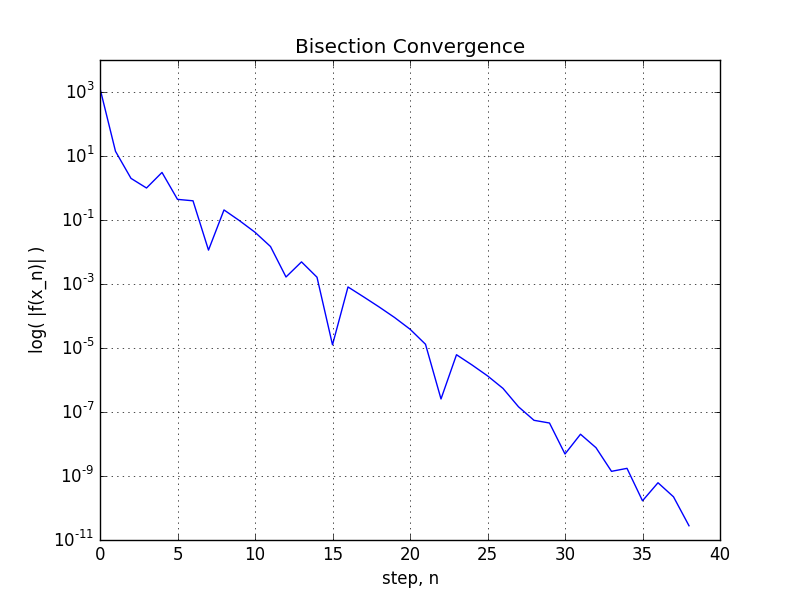
\includegraphics[width=0.5\textwidth]{Problem4a.png}
  %  \caption{(Approximately) Quadratic Convergence}
  %\end{figure}
 
  \section{Warmup}

  Consider a degree 3 and a degree 4 polynomial:

  \begin{align}
    \label{eq:poly3}
    A_1 &+ B_1x + C_1x^2+D_1x^3          \\
    \label{eq:poly4}
    A_2 &+ B_2x + C_2x^2+D_2x^3+E_2x^4
  \end{align}

  In order to intersect in five points, there must exist five solutions to the
  equation:

  \begin{equation}
    A_1+B_1x+C_1x^2+D_1x^3=A_2+B_2x+C_2x^2+D_2x^3+E_2x^4 \nonumber
  \end{equation}

  Rearranging makes it clear that there are only four possible soltions to the
  equation:
  
  \begin{equation}
    (A_1-A_2) + (B_1-B_2)x + (C_1-C_2)x^2 + (D_1-D_2)x^3 - E_2x^4 = 0 \nonumber
  \end{equation}

  Thus there can not be more than four intersections between two third and fourth
  polynomials.

  \section{Interpolation Accuracy}

  An interpolating polynomial for $ln(x)$ is obtained from a two degree Lagrange polynomial:

  \begin{align}
    L_3(x) &= y_1\frac{(x-x_2)(x-x_3)}{(x_1-x_2)(x_1-x_3)} + y_2\frac{(x-x_1)(x-x_3)}{(x_2-x_1)(x_2-x_3)} + y_3\frac{(x-x_1)(x-x_2)}{(x_3-x_1)(x_3-x_2)} \nonumber \\
    \label{eq:lninter}
    &= -ln2\frac{(x-1)(x-4)}{2} + ln4\frac{(x-1)(x-2)}{6}
  \end{align}

  \begin{figure}[h!]
    \centering
    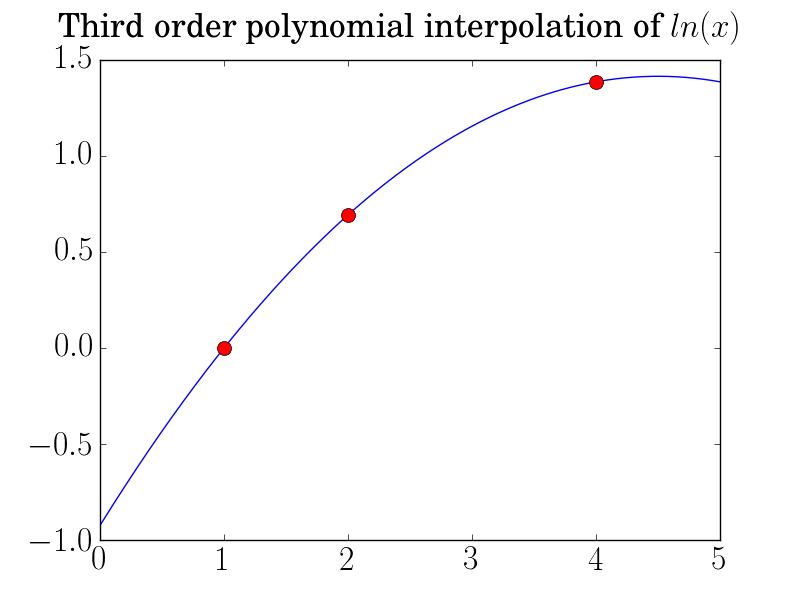
\includegraphics[width=0.5\textwidth]{Problem2.png}
    \caption{the interpolated function (eq \ref{eq:lninter}) for the given data points of $ln(x)$} 
  \end{figure}

  \clearpage

  \section{Bezier Curves}

  \begin{align}
    P_0 &= (1,1)            \nonumber \\
    P_1 &= (1,\frac{2}{3})  \nonumber \\
    P_2 &= (3,\frac{1}{3})  \nonumber \\
    P_3 &= (9,1)            \nonumber
  \end{align}

  \begin{figure}[h!]
    \centering
    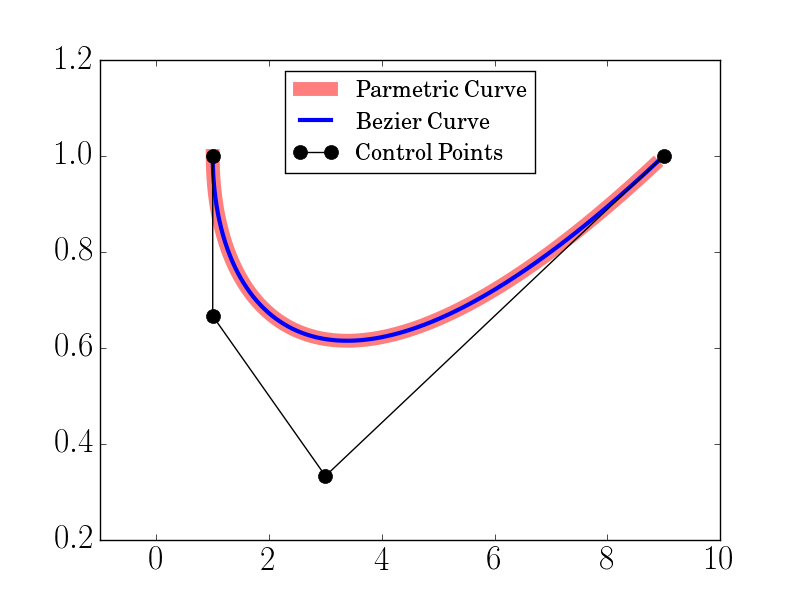
\includegraphics[width=0.7\textwidth]{Problem3.png}
    \caption{Piecewise function with its Bezier representation}
  \end{figure}

  \clearpage

  \section{Spline Theory}

  \begin{figure}[h!]
    \centering
    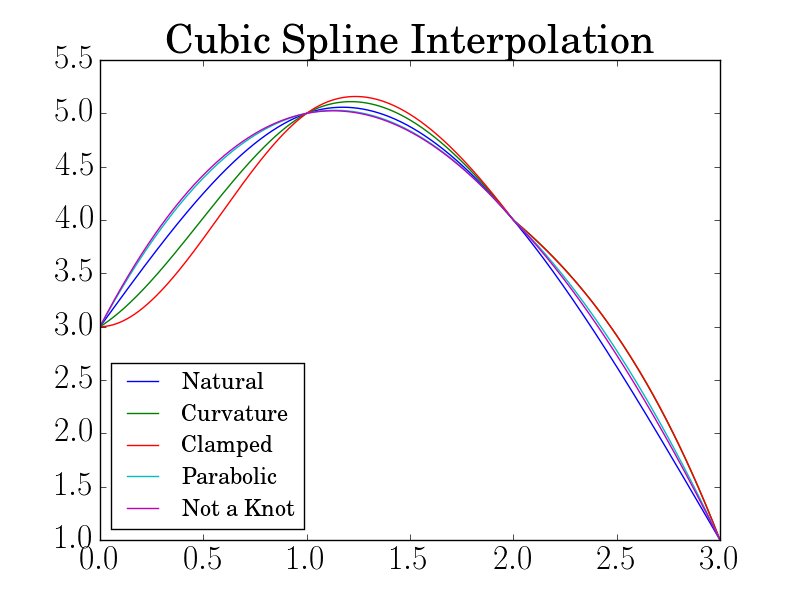
\includegraphics[width=0.7\textwidth]{spline.png}
    \caption{Cubic Spline Interpolation using different boundary conditions}
  \end{figure}

  \subsection*{Natural}
  $
    \bm{a} = \left[
  \begin{matrix}
  1 & 0 & 0 & 0 \\
  1 & 4 & 1 & 0 \\
  0 & 0.25  & 3.75 & 0 \\
  0 & 0 & 0 & 1
  \end{matrix}
  \right]
  \bm{x} = \left[
  \begin{matrix}
  0    \\
  -4 \\
  -2 \\
  0
  \end{matrix}
  \right]
  \bm{b} = \left[
  \begin{matrix}
  0   \\
  -18 \\
  -12 \\
  0
  \end{matrix}
  \right]
  $

  \subsection*{Curvature}
  Using $y_1^{\prime\prime}=5$, $y_4^{\prime\prime}=-5$

  $
  \bm{a} = \left[
  \begin{matrix}
  1 & 0 & 0 & 0 \\
  1 & 4 & 1 & 0 \\
  0 & 0.25 & 3.75 & 1 \\
  0 & 0 & 0 & 1
  \end{matrix}
  \right]
  \bm{x} = \left[
  \begin{matrix}
  5     \\
  -5.66 \\
  -0.33 \\
  -5
  \end{matrix}
  \right]
  \bm{b} = \left[
  \begin{matrix}
  5   \\
  -18 \\
  -12 \\
  -5
  \end{matrix}
  \right]
  $


  \subsection*{Clamped}
  Using $y_1^{\prime}=5$, $y_4^{\prime}=-5$

  $
  \bm{a} = \left[
  \begin{matrix}
  2 & 1 & 0 & 0 \\
  0.5 & 3.5 & 1 & 0 \\
  0 & 0.285 & 3.714 & 1 \\
  0 & 0 & 0.269 & 1.73
  \end{matrix}
  \right]
  \bm{x} = \left[
  \begin{matrix}
  -7.86    \\
  -2.26 \\
  --1.06 \\
  -5.46
  \end{matrix}
  \right]
  \bm{b} = \left[
  \begin{matrix}
  -18   \\
  -18 \\
  -12 \\
  -12
  \end{matrix}
  \right]
  $


  \subsection*{Parabolic}

  $
  \bm{a} = \left[
  \begin{matrix}
  1 & -1 & 0 & 0 \\
  1 & 5 & 1 & 0 \\
  0 & 0.2 & 3.8 & 1 \\
  0 & 0 & -0.263 & 1.263
  \end{matrix}
  \right]
  \bm{x} = \left[
  \begin{matrix}
  -3.25     \\
  -3.25 \\
  -1.75 \\
  -1.75
  \end{matrix}
  \right]
  \bm{b} = \left[
  \begin{matrix}
  0   \\
  -18 \\
  -12 \\
  0
  \end{matrix}
  \right]
  $

  \subsection*{Not-a-Knot}

  $
  \bm{a} = \left[
  \begin{matrix}
  1 & -2 & 1 & 0 \\
  1 & 6 & 0 & 0 \\
  0 & 0.166 & 4 & 1 \\
  0 & 0.166 & -0.5 & 1.5
  \end{matrix}
  \right]
  \bm{x} = \left[
  \begin{matrix}
  -4     \\
  -3        \\
  -2     \\
  -1
  \end{matrix}
  \right]
  \bm{b} = \left[
  \begin{matrix}
  0   \\
  -18 \\
  -12 \\
  0
  \end{matrix}
  \right]
  $


  \section{Runge's Phenomenon}

  Lagrange interpolating polynomials, natural cubic splines, and chebyshev
  polynomials were used to interpolate $1/(1+t^2)$. Error was evaluated using
  RMS error and tended to dercease for increasing numbers of points, as expected.
  The spline interpolation was best for all numbers of points in terms of the
  RMSE.

  \begin{table}[h!]
  \centering
  \begin{tabular}{| c | c | c | c |}
    \hline
    Method    & RMSE 5pt & RMSE 10pt & RMSE 15pt \\ \hline
    Lagrange  & 0.27918  & 0.10959   & 1.77154   \\
    Splines   & 0.14108  & 0.04083   & 0.00075   \\
    Chebyshev & 0.22641  & 0.07909   & 0.02549   \\ \hline
  \end{tabular}
  \end{table}


  \begin{align}
    f(t)=\frac{1}{1+t^2}
  \end{align}

  \begin{figure}[h!]
    \centering
    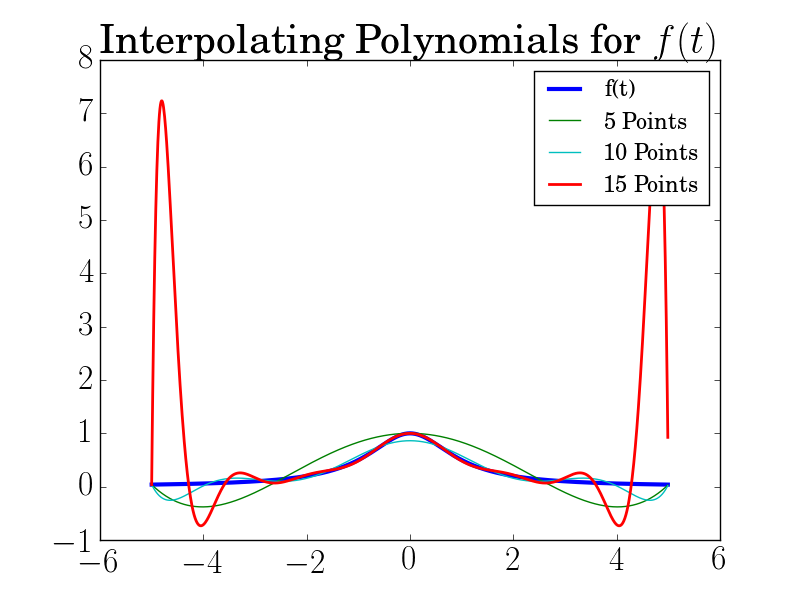
\includegraphics[width=0.7\textwidth]{Problem5i.png}
    \caption{Lagrange Interpolating Polynomials}
  \end{figure}

  \begin{figure}[h!]
    \centering
    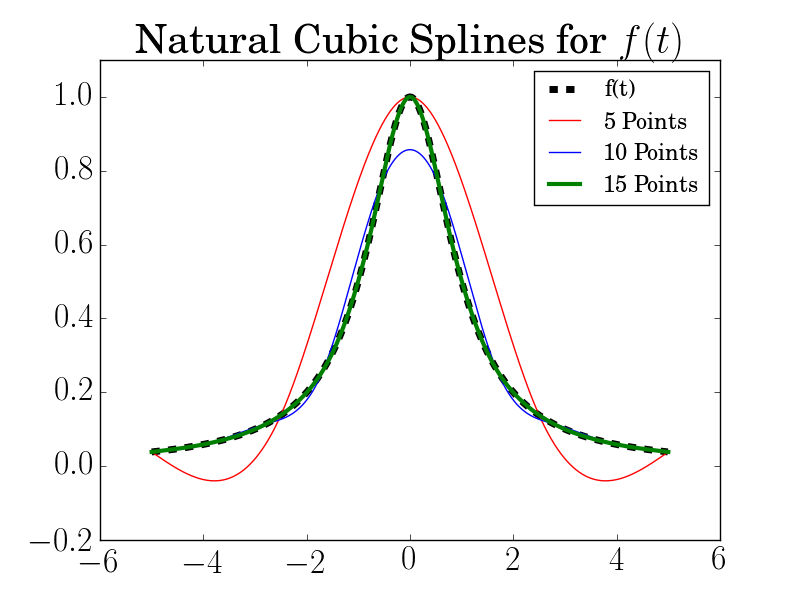
\includegraphics[width=0.7\textwidth]{Problem5ii.png}
    \caption{Natural cubic spline interpolation for varying numbers of sample points}
  \end{figure}

  \begin{figure}[h!]
    \centering
    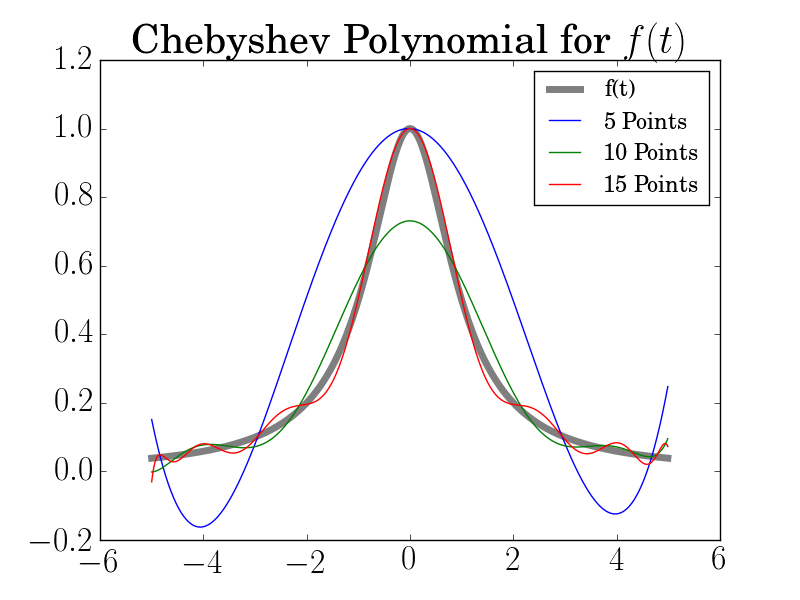
\includegraphics[width=0.7\textwidth]{Problem5iii.png}
    \caption{Chebyshev Polynomial for varying numbers of sample points.}
  \end{figure}

  

  \clearpage 

  \section{Gibb's Phenomenon}
 
   
  \begin{figure}[h!]
    \centering
    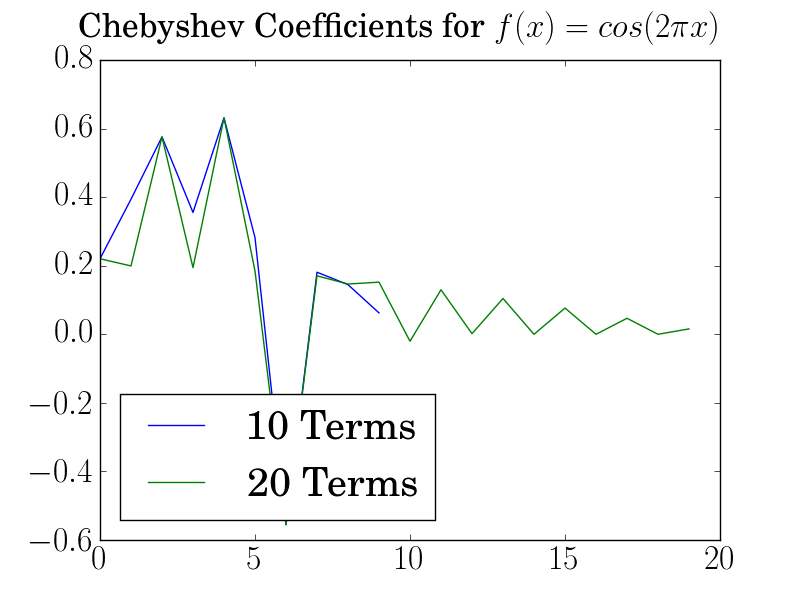
\includegraphics[width=0.7\textwidth]{Problem6ia.png}
    \caption{Ringing phenomenon in Chebyshev approximations}
  \end{figure}

  \begin{figure}[h!]
    \centering
    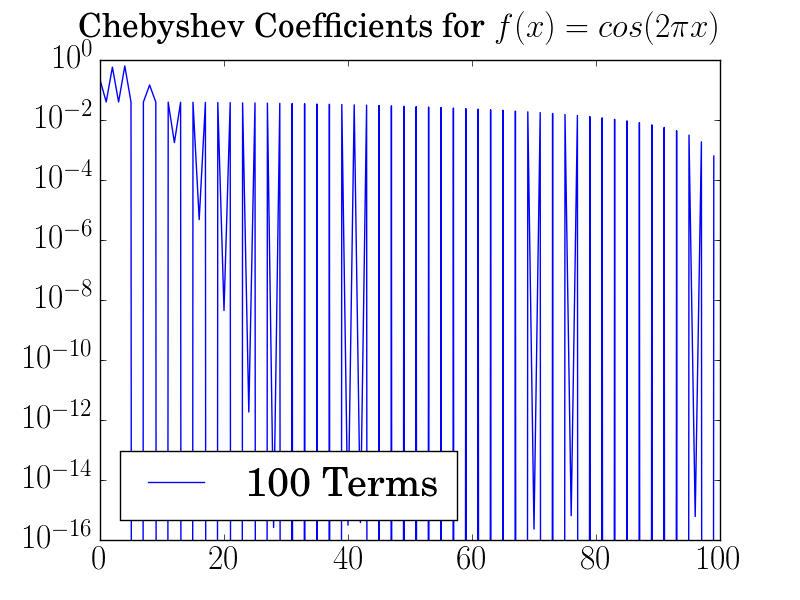
\includegraphics[width=0.7\textwidth]{Problem6ib.png}
    \caption{100 Coefficients displaying a clear power law relationship}
  \end{figure}
 
   
  \begin{figure}[h!]
    \centering
    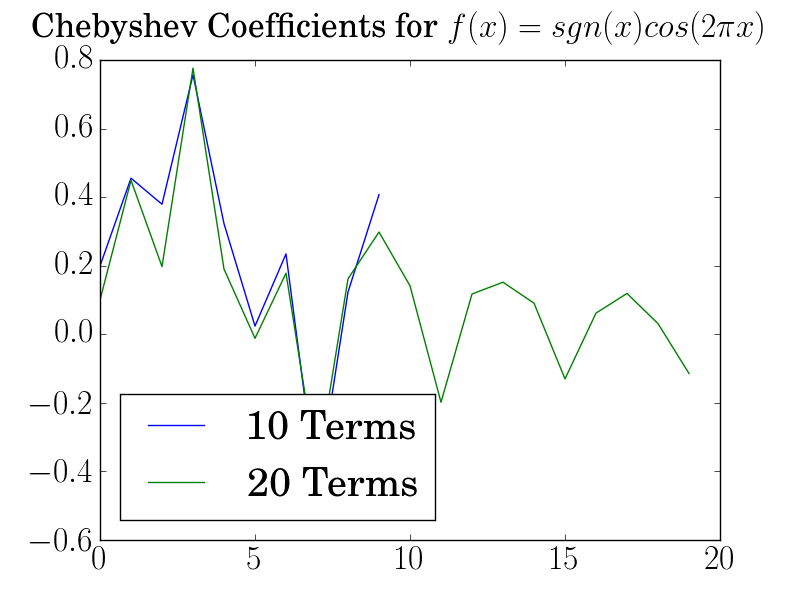
\includegraphics[width=0.7\textwidth]{Problem6iia.png}
    \caption{Ringing phenomenon in Chebyshev approximations}
  \end{figure}

  \begin{figure}[h!]
    \centering
    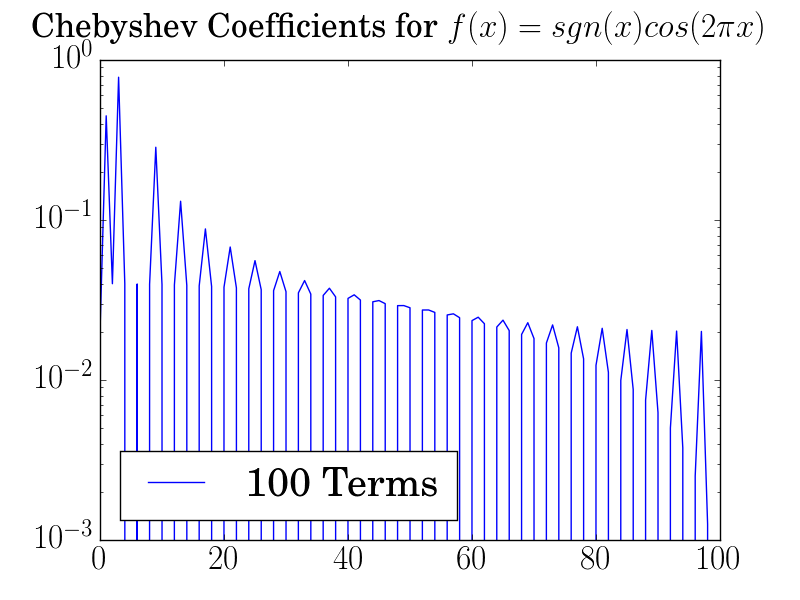
\includegraphics[width=0.7\textwidth]{Problem6iib.png}
    \caption{100 Coefficients displaying a clear power law relationship}
  \end{figure}
 
   
  \begin{figure}[h!]
    \centering
    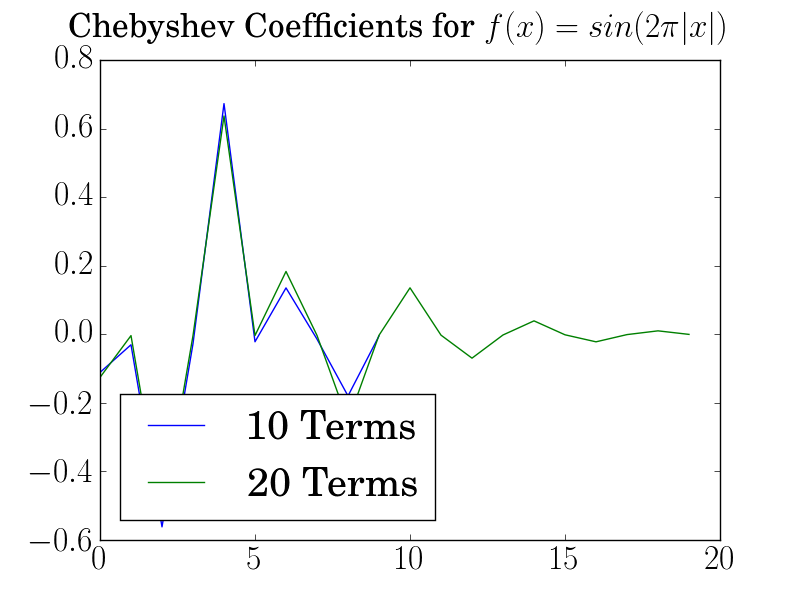
\includegraphics[width=0.7\textwidth]{Problem6iiia.png}
    \caption{Ringing phenomenon in Chebyshev approximations}
  \end{figure}

  \begin{figure}[h!]
    \centering
    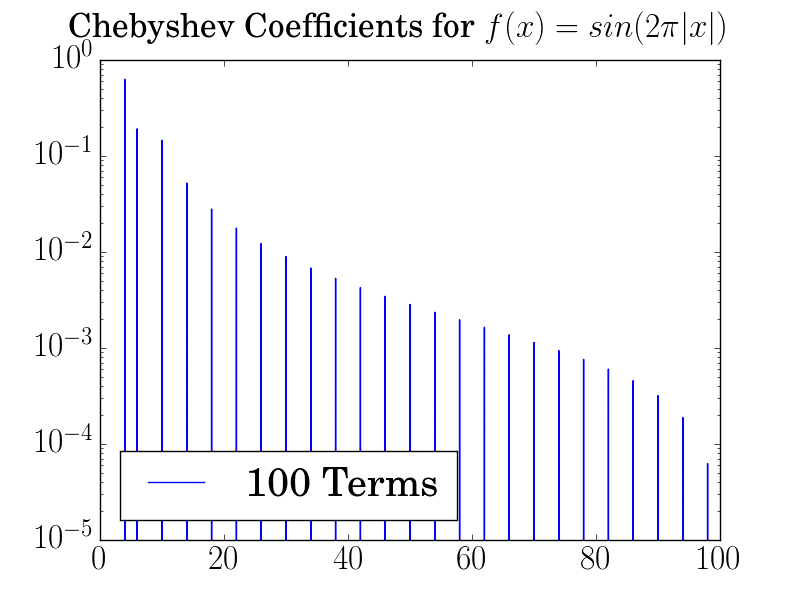
\includegraphics[width=0.7\textwidth]{Problem6iiib.png}
    \caption{100 Coefficients displaying a clear power law relationship}
  \end{figure}

  \clearpage

  \section{Chebyshev Calculus}


  \subsection{First Derivatives}
  \begin{align}
    T_{10}^\prime(x) &= 100x-1600x^3+6720*x^5-10240*x^7+5120*x^9 \nonumber \\
    T_{15}^\prime(x) &= -15+1680*x^2-30240*x^4-633600x^8+1013760x^{10}-798720x^{12}+245760x^{14} \nonumber \\
    T_{20}^\prime(x) &= -400x+26400x^3-506880x^5+4392960x^7-20500480x^9+55910400x^{11}\\&-91750400x^{13}+89128960x^{15}-47185920x^{17}+10485760x^{19} \nonumber
  \end{align}  

  \subsection{Second Derivatives}
  \begin{align}
    T_{10}^{\prime\prime}(x) &= 100-4800x^2+33600x^4-71680x^6+46080x^8 \nonumber \\
    T_{15}^{\prime\prime}(x) &= 3360x-120960x^3+1209600x^5-5068800x^7+10137600x^9-9584649x^{11}+3440640x^{13} \nonumber\\
    T_{20}^{\prime\prime}(x) &= -400+79200x^2+30750720x^6-184504320x^8+615014400x^{10}-\\&1192755200x^{12}+1336934400x^{14}-802160640x^{16}+199229440x^{18} \nonumber
  \end{align}  

  \subsection{Integral}
  \begin{align}
    \int T_{10}(x)dx &= -x+\frac{50}{3}-80x^5+160x^7-\frac{1280}{9}x^9+\frac{512}{11}x^{11} \nonumber \\
    \int T_{15}(x)dx &= -\frac{15}{2}x^2+140x^4-1008x^6+3600x^8-7040x^{10}+7680x^{12}-\frac{30720}{7}x^{14}+1024x^{16} \nonumber \\
    \int T_{20}(x)dx &= \frac{200}{3}x^3+1320x^5-\frac{84480}{7}x^7+\frac{183040}{3}x^9-\\&186368x^{11}+358400x^{13}-\frac{1310720}{3}x^{15}+327680x^{17}-\frac{2621440}{19}x^{19}+\frac{524288}{21}x^{21} \nonumber
  \end{align}

  \section{Cephied Lightcurve}

  The spline fit is much more reasonable for the edge cases compared to the Lagrange
  polynomial.

  \begin{figure}[h!]
    \centering
    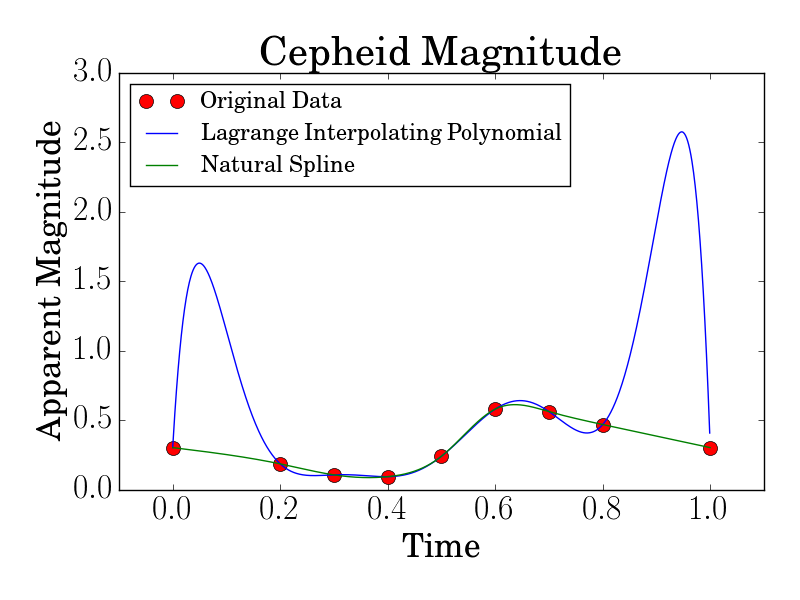
\includegraphics[width=0.9\textwidth]{Problem8.png}
  \end{figure}

  
    
  
\end{document}
